\documentclass[10pt,a4paper]{article}

\usepackage[margin=2.5cm]{geometry}
\usepackage[utf8]{inputenc}
\usepackage[danish]{babel}
\usepackage{graphicx}
\usepackage{subfig}
\usepackage{listings}
\usepackage{tikz}
\usepackage{fancyvrb}
\usepackage{hyperref}


\renewcommand{\FancyVerbSpace}{\textcolor{lightgray}{.}}


\usetikzlibrary{calc}

\lstset{
  numbers=left,
  numberstyle=\tiny\color{gray},
  basicstyle=\small\ttfamily,
  aboveskip=0pt,
  belowskip=0pt
}

\title{\textsc{\Huge Ricochet Robots}\\\textsc{Programmeringskonkurrence}\\[0.25cm]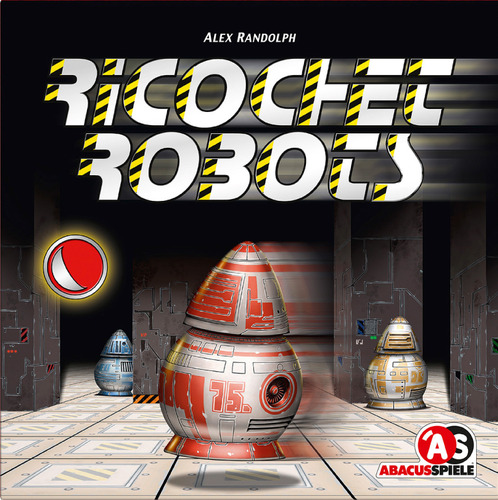
\includegraphics[height=3cm]{img/boxart.jpg}}
\date{}
\author{{\small Forfattere: Asger Juul Brunshøj, Anders Roy Christiansen, Signe Colding-Jørgensen,}\\{\small Andreas Halkjær From, Marcus Skov Hansen, Lasse Kokholm, Gandalf Saxe og Hjalte Wedel Vildhøj.}}
\begin{document}

\maketitle

\section{Introduktion}
Formålet med denne konkurrence er at designe og implementere et program, der kan spille brætspillet \emph{Ricochet Robots}. De indsendte programmer bliver sat til at dyste mod hinanden, og gruppen, der har lavet det bedste program vinder selvfølgelig en præmie!

Man kan deltage i konkurrencen i grupper bestående af op til fire studerende, og deltagelse tæller som en bestået obligatorisk afleveringsopgave for alle gruppemedlemmer. Der skal ikke skrives nogen rapport. Flere praktiske informationer findes sidst i dette dokument. Bemærk dog følgende vigtige datoer:

\begin{description}
\item [7. april kl. 12.30-14.30] Kom-og-kod-workshop med Signe  Colding-Jørgensen, Andreas H. From og kage. Her vil det være muligt at få hjælp og diskutere sin løsning med andre. Sted: Bygning 324/040.
\item [6. maj kl. 20.00:] Deadline for at uploade sit program til CodeJudge.
\item [12. maj kl. 10.30:] Præmieoverrækkelse. Resultatet af konkurrencen præsenteres og vinderne annonceres. Sted: Bygning 116/81.
\end{description}


\subsection{Kort om brætspillet}
I Ricochet Robots gælder det om at bevæge brikker (kaldet \emph{robotter}) rundt på en forudbestemt bane, så en bestemt robot (fx den grønne) ender på en bestemt position (Se Figur~\ref{FIG:REALS}). En robot kan på et træk bevæge sig enten op, ned, til venstre eller til højre, hvormed den fortsætter i den valgte retning indtil den støder på en mur, en anden robot eller banens kant. Det gælder om at få robotten til at ende på målfeltet med færrest mulige samlede træk, altså inklusive træk med eventuelle andre robotter. For at opnå en løsning med få træk, er det meget ofte en fordel (og nogle gange også nødvendigt) at flytte andre robotter end den robot, der skal hen på målet.

%går ud på at bevæge visse brikker (kaldet \emph{robotter}) rundt på et forudbestemt bræt (herefter kaldet \emph{banen}) for at opnå specifikke positioner (herefter kaldet \emph{nøgler}) i så få samlede træk som muligt med visse bevægelsesmæssige begrænsninger.

\begin{figure}[h]
\centering
%\hfill
%\subfloat{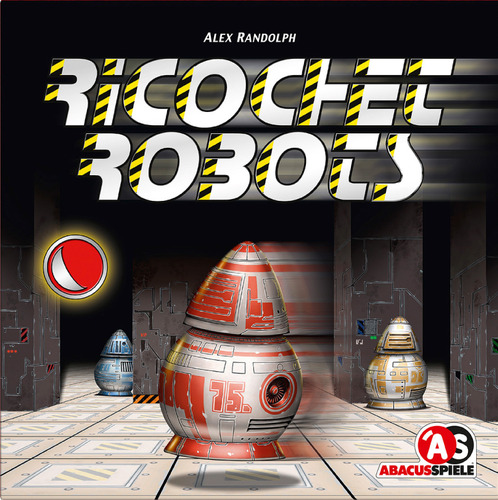
\includegraphics[height=4cm]{img/boxart.jpg}}
\hfill
\subfloat{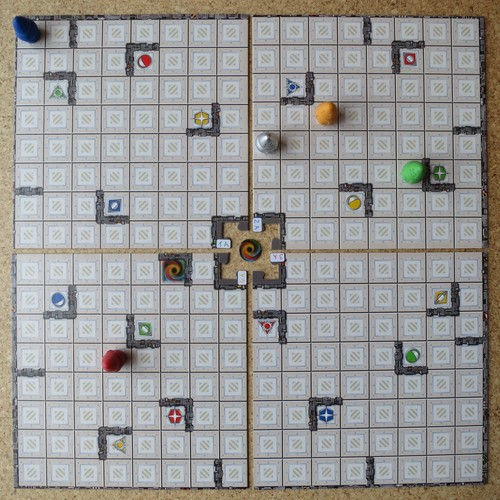
\includegraphics[height=4cm]{img/realboard.jpg}}
%\quad
%\subfloat[Repræsentation]{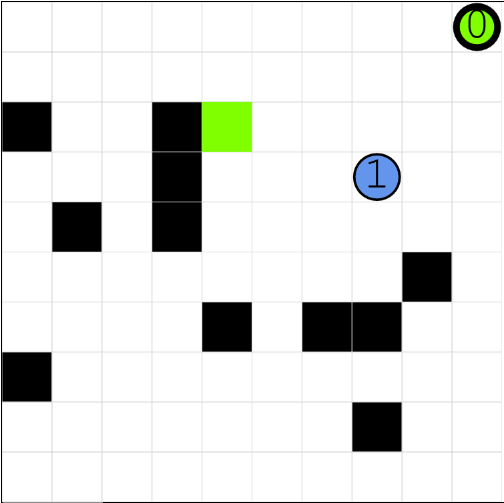
\includegraphics[height=4cm]{img/representation.png}}
%\quad
%\subfloat[Filformat]{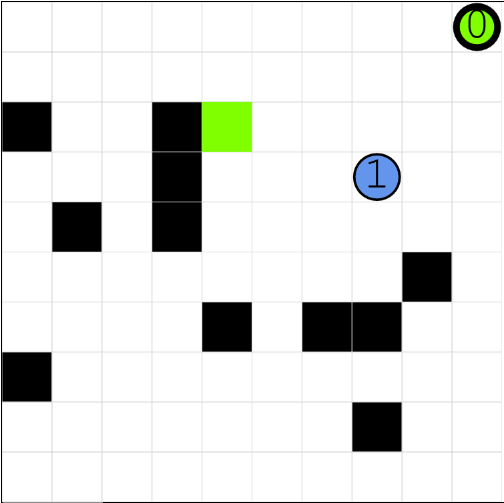
\includegraphics[height=4cm]{img/representation.png}}
\hfill
~
\caption{Brætspillet Ricochet Robots}
\label{FIG:REALS}
\end{figure}

\newsavebox{\simpleboard}
\begin{lrbox}\simpleboard%
\hspace{1cm}
\begin{minipage}[b]{2.1cm}%
\begin{Verbatim}[frame=single, numbers=left,showspaces, commandchars=\\\{\}, baselinestretch=0.64]
10
2
         0\phantom{}
   ##     \phantom{}
#  #G     \phantom{}
   #   1  \phantom{}
 # #      \phantom{}
        # \phantom{}
      ##  \phantom{}
#  #      \phantom{}
       #  \phantom{}
          \phantom{}
          \phantom{}
\end{Verbatim}%
\end{minipage}
\hspace{1cm}
\end{lrbox}

\newsavebox{\simpleboardsolution}
\begin{lrbox}\simpleboardsolution%
\hspace{1cm}
\begin{minipage}[b]{2.1cm}%
\begin{Verbatim}[frame=single, numbers=left,showspaces, commandchars=\\\{\}, baselinestretch=0.64, label={\scriptsize Løsning 1}]
0D
0L
0U
0R
0U
0L
0U
\end{Verbatim}
\vspace{-4pt}
\begin{Verbatim}[frame=single, numbers=left,showspaces, commandchars=\\\{\}, baselinestretch=0.64, label={\scriptsize Løsning 2}]
1R
0D
0L
\end{Verbatim}%
\end{minipage}
\hspace{1cm}
\end{lrbox}

\begin{figure}
\centering
\subfloat[Brættet \texttt{2-simpleboard.txt}. De grå prikker er mellemrum.\label{fig:simpleboardfile}]{
\usebox\simpleboard
}
\hspace{0.2cm}
\subfloat[Visualisering af \texttt{2-simpleboard.txt}.\label{fig:simpleboardgui}]{
\begin{minipage}[b]{5cm}
  \centering
  \begingroup\fboxsep=0pt
  \fbox{\href{test}{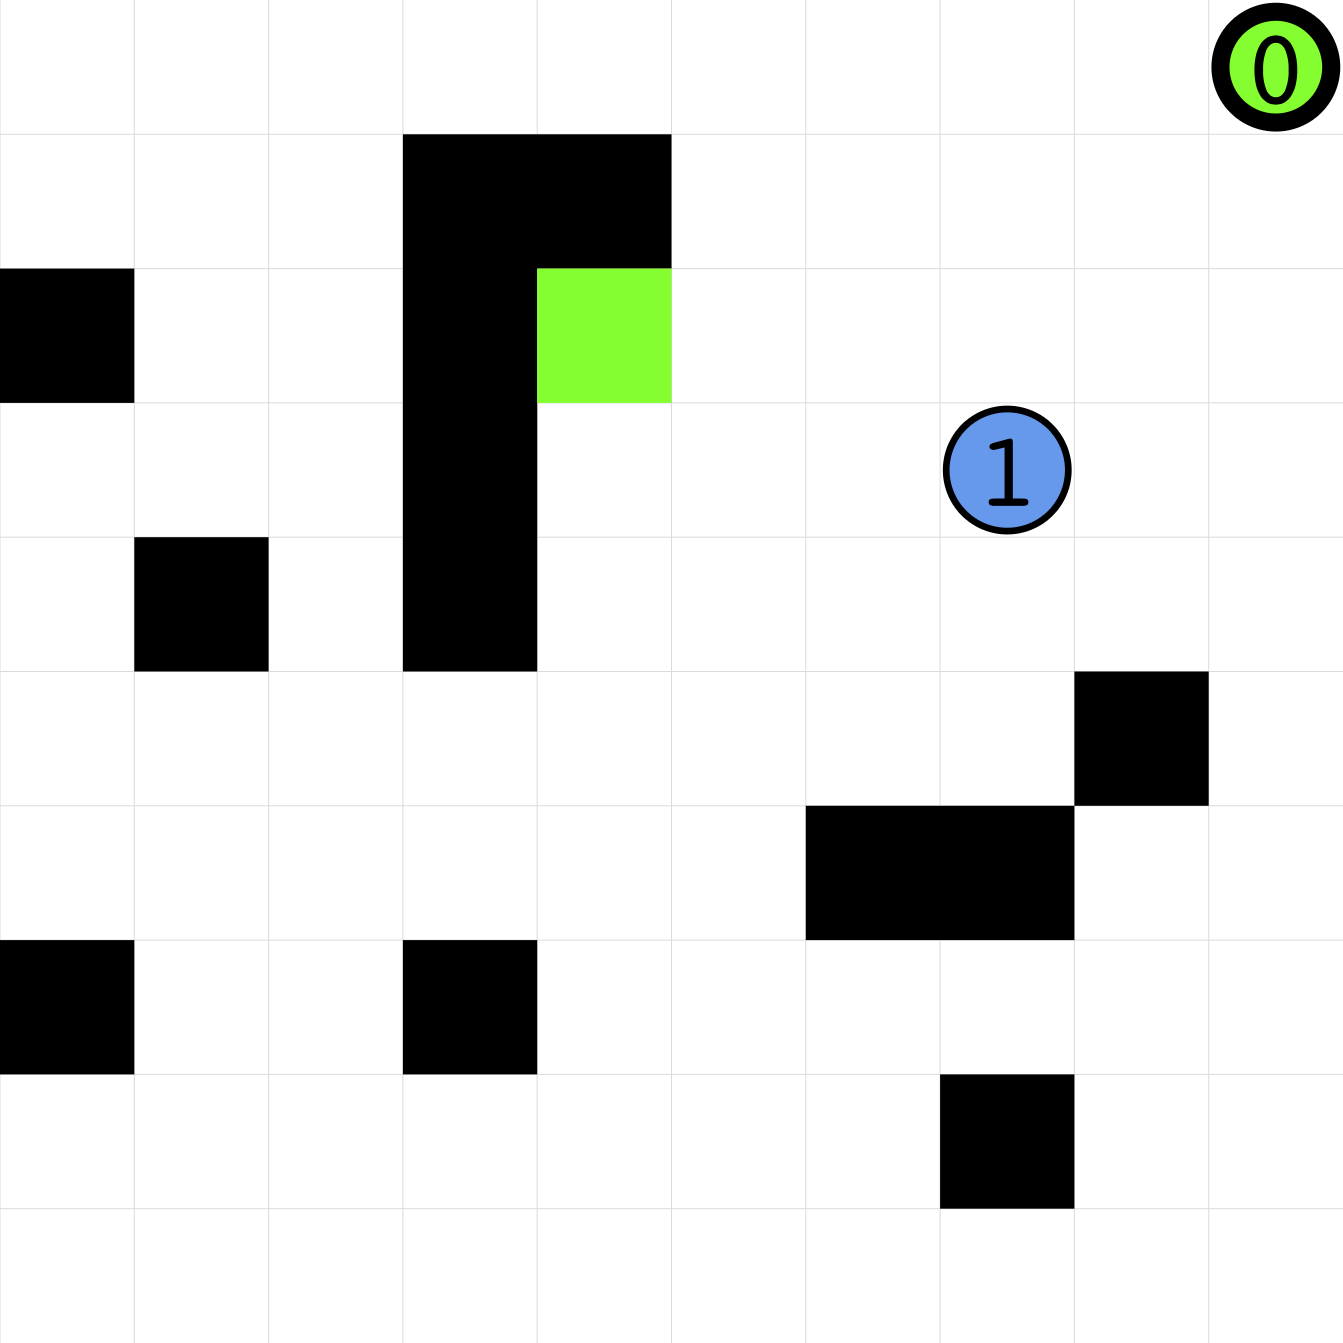
\includegraphics[height=4cm]{img/2-simpleboard.png}}}
  \endgroup
\end{minipage}
}
\hspace{0.2cm}
\subfloat[To gyldige løsninger af henholdsvis længde 7 og 3.\label{fig:simpleboardsolutions}]{
  \usebox\simpleboardsolution
}
\caption{Eksempel på en bane af størrelse $n=10$ med $r=2$ robotter. De sorte felter er vægge og det grønne felt er målfeltet for robot 0. Den optimale løsning til denne bane har længde 3.}
\label{fig:simpleboardexample}
\end{figure}

\section{Konkurrencen}
I konkurrencen vil vi arbejde med en forsimplet version af brætspillet, der bevarer spillets unikke udfordringer. Denne version spilles på et kvadratisk gitter (kaldet banen) bestående af $n \times n$ felter, hvor $2 \leq n \leq 1000$. I banen findes $r$ robotter, hvor $1 \leq r \leq 10$. Robotterne er nummeret $0, \ldots, r-1$, og det gælder altid om at få robot 0 hen på det unikke målfelt. Robotterne bevæger sig som i brætspillet og stopper således først når de rammer en væg, en anden robot eller banens kant. \textbf{Bemærk, at robot 0 skal stå stille på målet for at banen er løst!}

Figur~\ref{fig:simpleboardexample} viser et eksempel på en bane med $n=10$ og $r=2$ samt to mulige løsninger. I de næste to sektioner beskrives det formelle input- og outputformat samt kravene til jeres program.

\subsection{Inputformat}
Inputtet til jeres program er en bane som vist i Figur~\ref{fig:simpleboardfile}. Den første linje angiver banestørrelsen $n$ som et heltal mellem $2$ og $1000$. Den anden linje angiver antallet af robotter $r$ som et heltal mellem $1$ og $10$. De efterfølgende $n$ linjer angiver banen. Hver af disse linjer består af $n$ symboler, der repræsenterer indholdet på denne position i banen. De lovlige symboler i en linje er:

\begin{description}
\item[\texttt{\#}]: Angiver at positionen er en væg.
\item[(mellemrum)]: Angiver at positionen er tom.
\item[\texttt{G}]: Angiver at positionen er målpositionen for robot 0.
\item[\texttt{0, 1}, \ldots, $(r-1)$]: Angiver at robotten med dette tal er på denne position.
\end{description}
Det garanteres, at symbolet \texttt{G} og robotterne \texttt{0, 1}, $\ldots (r-1)$ optræder på præcis én position i banen. Det garanteres desuden at banen kan løses.

\subsection{Outputformat}
En gyldig løsning til banen er en sekvens af træk, der bringer robot 0 hen og i hvile på målpositionen. Hvert træk udskrives som en linje bestående af præcis to symboler: Et heltal $i$, hvor $0 \leq i \leq r-1$, efterfulgt (uden mellemrum) af et af symbolerne \texttt{R} (højre), \texttt{L} (venstre), \texttt{U} (op) eller \texttt{D} (ned). Fx angiver \texttt{0R} at robot 0 flyttes mod højre. Et eksempel på to gyldige løsninger er vist i Figur~\ref{fig:simpleboardsolutions}.

\subsection{Krav til jeres program}
Jeres program skal indlæse en bane fra konsollen (std.in), beregne en gyldig løsning og udskrive denne løsning til konsollen (std.out). Det er ikke et krav at jeres program finder den korteste løsning, men jo kortere løsningen er, desto flere points får jeres program.


%\item 
%\item Spillet slutter 

% få robot 0 robot (markeret med grønt) 
%\end{itemize}


\section{Sådan kommer du igang -- og anden praktisk information}

Start med at hente filen \texttt{rr.zip}, der ligger på CampusNet under fildeling. Filen indeholder en skabelon i hhv. Java og C++ med forskellige brugbare metoder til fx indlæsning af banefiler m.m. Prøv at uploade filen \texttt{Ricochet.java} til CodeJudge -- så burde den klare den første test.

Det er ikke et krav at tage udgangspunkt i disse skabeloner -- I må også meget gerne skrive jeres løsning i andre sprog, der er understøttede på CodeJudge.

Filen \texttt{rr.zip} indeholder desuden en række forskellige baner, som I kan teste jeres løsning på. Alle banefilnavne starter med et tal, der angiver, hvor mange robotter, der er i banen.

Herunder følger yderligere relevant information.

%Det er tilladt at samarbejde på konkurrencen i grupper på op til fire studerende. Det kan i øvrigt på det kraftigste anbefales at deltage i konkurrencen uanset ambitionsniveau, da arbejdet med problemerne unægteligt vil forbedre jeres forudsætninger for den endelige eksamen.

%Derudover vil vi lade en vilkårlig besvarelse på konkurrencen, som blot passerer de første fem prøver lagt op på CodeJudge, tælle som en bestået obligatorisk afleveringsopgave for hvert gruppemedlem, hvilket er en ekstra chance for at kunne gå til den endelige eksamen. Endelig vil der være en præmie til gruppen med den bedste løsning.

\paragraph{Piazza} Brug Piazza til alle spørgsmål, der ikke er besvaret her.

\paragraph{Gruppedannelse} Husk at danne gruppe på CodeJudge. Maksimum er fire studerende per gruppe. Aflevering foregår ved at uploade sin løsning til CodeJudge.

\paragraph{CodeJudge} Konkurrencen foregår på CodeJudge og er opdelt i to delopgaver: \emph{Obligatorisk} og \emph{Konkurrence}. Den obligatoriske del består af forholdsvis nemme baner med en enkelt robot. Start med at lave en løsning til denne del. Konkurrencedelen indeholder større og mere udfordrende baner med op til 10 robotter.

\paragraph{Den obligatoriske del} Uploades en løsning, der består alle tests (5 synlige og 5 skjulte) i den obligatoriske del, tæller dette som en bestået obligatorisk afleveringsopgave for alle medlemmer af gruppen.

\paragraph{Konkurrencedelen} Efter deadline tager vi den nyeste version af jeres program i konkurrencedelen og lader det dyste mod de andre programmer på en ukendt samling af baner.

\paragraph{Tids- og hukommelsesgrænser} På CodeJudge bliver jeres program tildelt $T$ sekunders CPU-tid og $S$ MB hukommelse. I kan læse værdierne $T$ og $S$ som de første to kommandolinjeargumenter til jeres program. Som udgangspunkt kan I regne med at $T=5$ sekunder og $S=500$MB, men når den endelige konkurrence afvikles efter deadline, bliver jeres program tildelt en del flere resourcer.

\paragraph{Pointtildeling} For hver bane i konkurrencedelen som jeres program løser får det $100 \frac{E}{U}$ points, hvor $U$ er længden af jeres løsning, og $E$ er et estimat af den bedst mulige løsning for banen.

\paragraph{Scoreboard} På Scoreboardet på CodeJudge kan man løbende følge med i, hvordan ens løsning klarer sig i forhold til andre gruppers løsninger. Grupperne er sorteret efter det totale antal points deres løsning har opnået på konkurrencebanerne. I tilfælde af pointlighed er den bedste gruppe den med det korteste tidsforbrug. Bemærk, at vi til den endelige konkurrence også tester jeres program på nye og ukendte baner, så derfor er det ikke sikkert, at den endelige vinder bliver den gruppe, der ligger øverst på Scoreboardet.

\paragraph{Webapp} På hjemmesiden \url{https://hwv.dk/rr/} findes en app, hvor man kan importere/eksportere baner og løsninger -- og selv prøve at spille banen vha. tastaturet eller mus/touch. Man kan også komme direkte til denne app ved at klikke på visualiseringen af en bane i CodeJudge. Appen er kun testet i Chrome og Safari, men burde også virke i andre browsere og på tablets og touchenheder. Bugs kan mailes til Hjalte på \href{mailto:hwv@hwv.dk}{\texttt{hwv@hwv.dk}}.

\paragraph{Nogle gode råd} Start med at lave en løsning, der virker for helt små baner, hvor der kun er en robot. Overvej, hvordan du kan bruge algoritmiske redskaber fra kurset som fx bredde-først-søgning og hashing til at søge efter en løsning.

\begin{figure}
\centering
\href{https://hwv.dk/rr/#%7B%22board%22%3A%2237%5Cn10%5Cn%23%23%23%23%23%23%23%23%23%23%23%23%23%23%23%23%23%23%23%23%23%23%23%23%23%23%23%23%23%23%23%23%23%23%23%23%23%5Cn%23456%23%20%23%20%23%20%23%20%23%20%23%20%20%20%23%20%20%20%20%20%20%20%20%20%20%20%23%20%20%20%20%20%23%5Cn%233%237%23%20%23%20%23%20%23%20%23%20%23%20%23%20%23%23%23%20%23%20%23%23%23%23%23%20%23%23%23%20%23%20%23%5Cn%232%238%23%20%20%20%20%20%20%20%23%20%23%20%23%20%20%20%23%20%23%20%23%20%23%20%23%20%23%20%20%20%23%20%23%5Cn%231%239%23%20%23%23%23%23%23%23%23%20%23%20%23%23%23%23%23%20%23%23%23%20%23%20%23%23%23%23%23%20%23%23%23%5Cn%230%23%20%20%20%20%20%20%20%20%20%23%20%20%20%20%20%23%20%20%20%20%20%23%20%23%20%20%20%23%20%20%20%20%20%23%5Cn%23%23%23%23%23%23%23%23%23%20%23%20%23%23%23%23%23%20%23%23%23%20%23%23%23%20%23%20%23%20%23%23%23%20%23%20%23%5Cn%23%20%23%20%23%20%20%20%20%20%23%20%23%20%20%20%20%20%23%20%20%20%20%20%20%20%23%20%23%20%20%20%23%20%23%20%23%5Cn%23%20%23%20%23%23%23%20%23%23%23%20%23%23%23%20%23%20%23%20%23%20%23%23%23%20%23%20%23%23%23%23%23%20%23%23%23%5Cn%23%20%23%20%20%20%20%20%20%20%23%20%23%20%20%20%23%20%23%20%23%20%23%20%23%20%20%20%23%20%20%20%20%20%20%20%23%5Cn%23%20%23%23%23%20%23%20%23%20%23%20%23%20%23%20%23%23%23%23%23%23%23%20%23%20%23%20%23%23%23%23%23%20%23%23%23%5Cn%23%20%20%20%20%20%23%20%23%20%23%20%23%23%23%20%23%20%23%20%23%20%20%20%20%20%23%20%20%20%20%20%20%20%23%20%23%5Cn%23%23%23%20%23%20%23%23%23%23%23%20%20%20%20%20%23%20%23%20%23%20%23%20%23%23%23%20%23%23%23%20%23%20%23%20%23%5Cn%23%20%20%20%23%20%23%20%20%20%23%20%23%20%23%20%23%20%20%20%23%20%23%20%23%20%23%20%23%20%20%20%23%20%23%20%23%5Cn%23%20%23%20%23%23%23%20%23%23%23%23%23%20%23%20%23%20%23%23%23%23%23%23%23%20%23%23%23%20%23%23%23%20%23%20%23%5Cn%23%20%23%20%20%20%23%20%20%20%20%20%23%20%23%20%20%20%20%20%23%20%20%20%20%20%20%20%23%20%20%20%23%20%23%20%23%5Cn%23%23%23%23%23%20%23%23%23%20%23%23%23%23%23%20%23%23%23%20%23%20%23%20%23%23%23%20%23%20%23%23%23%23%23%20%23%5Cn%23%20%23%20%20%20%23%20%23%20%20%20%23%20%23%20%23%20%20%20%20%20%23%20%23%20%20%20%20%20%20%20%20%20%23%20%23%5Cn%23%20%23%20%23%20%23%20%23%20%23%23%23%20%23%20%23%23%23%20%23%23%23%23%23%20%23%23%23%20%23%23%23%23%23%20%23%5Cn%23%20%20%20%23%20%20%20%20%20%20%20%20%20%20%20%23%20%23%20%20%20%23%20%23%20%23%20%20%20%20%20%23%20%20%20%23%5Cn%23%23%23%23%23%20%23%23%23%23%23%23%23%23%23%20%23%20%23%23%23%20%23%20%23%23%23%23%23%20%23%23%23%20%23%20%23%5Cn%23%20%20%20%20%20%23%20%20%20%20%20%20%20%23%20%20%20%20%20%20%20%23%20%20%20%20%20%20%20%20%20%23%20%23%20%23%5Cn%23%20%23%23%23%20%23%20%23%23%23%23%23%20%23%20%23%23%23%23%23%20%23%23%23%23%23%23%23%20%23%20%23%23%23%20%23%5Cn%23%20%23%20%20%20%23%20%20%20%20%23%20%20%23%20%20%20%23%20%23%20%20%20%23%20%20%20%20%20%23%20%20%20%23%20%23%5Cn%23%20%23%23%23%23%23%23%23%23%20%23%23%20%23%23%23%23%23%20%23%23%23%23%23%23%23%23%23%20%23%23%23%23%23%20%23%5Cn%23%20%23%20%20%20%20%20%23%20%20%20%23%20%20%20%23%20%20%20%23%20%20%20%20%20%23%20%20%20%20%20%23%20%20%20%23%5Cn%23%20%23%23%23%23%23%20%23%20%23%23%23%23%23%20%23%23%23%20%23%23%23%20%23%20%23%23%23%20%23%23%23%20%23%23%23%5Cn%23%20%20%20%23%20%20%20%20%20%20%20%20%20%23%20%20%20%20%20%23%20%20%20%23%20%20%20%23%20%23%20%20%20%20%20%23%5Cn%23%23%23%20%23%20%23%23%23%23%23%23%23%23%23%23%23%20%23%23%23%20%23%23%23%23%23%20%23%23%23%20%23%23%23%20%23%5Cn%23%20%20%20%20%20%23%20%20%20%20%20%20%20%20%20%23%20%20%20%23%20%20%20%23%20%23%20%20%20%20%20%23%20%23%20%23%5Cn%23%20%23%23%23%20%23%23%23%23%23%20%23%23%23%23%23%20%23%20%23%20%23%23%23%20%23%23%23%20%23%20%23%20%23%20%23%5Cn%23%20%20%20%23%20%20%20%20%20%20%20%20%20%23%20%20%20%23%20%20%20%23%20%20%20%20%20%20%20%23%20%23%20%20%20%23%5Cn%23%23%23%20%23%23%23%23%23%23%23%20%23%23%23%23%23%20%23%23%23%23%23%23%23%20%23%23%23%20%23%23%23%23%23%20%23%5Cn%23%20%23%20%23%20%20%20%23%20%20%20%23%20%20%20%23%20%23%20%20%20%20%20%23%20%23%20%23%20%23%20%20%20%20%20%23%5Cn%23%20%23%23%23%20%23%23%23%20%23%23%23%20%23%20%23%20%23%20%23%23%23%20%23%23%23%20%23%20%23%23%23%20%23%20%23%5Cn%23%20%20%20%20%20%20%20%20%20%20%20%20%20%23%20%20%20%20%20%23%20%20%20%20%20%20%20%23%20%23%20%20%20%23%20G%5Cn%23%23%23%23%23%23%23%23%23%23%23%23%23%23%23%23%23%23%23%23%23%23%23%23%23%23%23%23%23%23%23%23%23%23%23%23%23%5Cn%22%2C%22moves%22%3A%22%22%2C%22pastMoves%22%3A0%7D}{
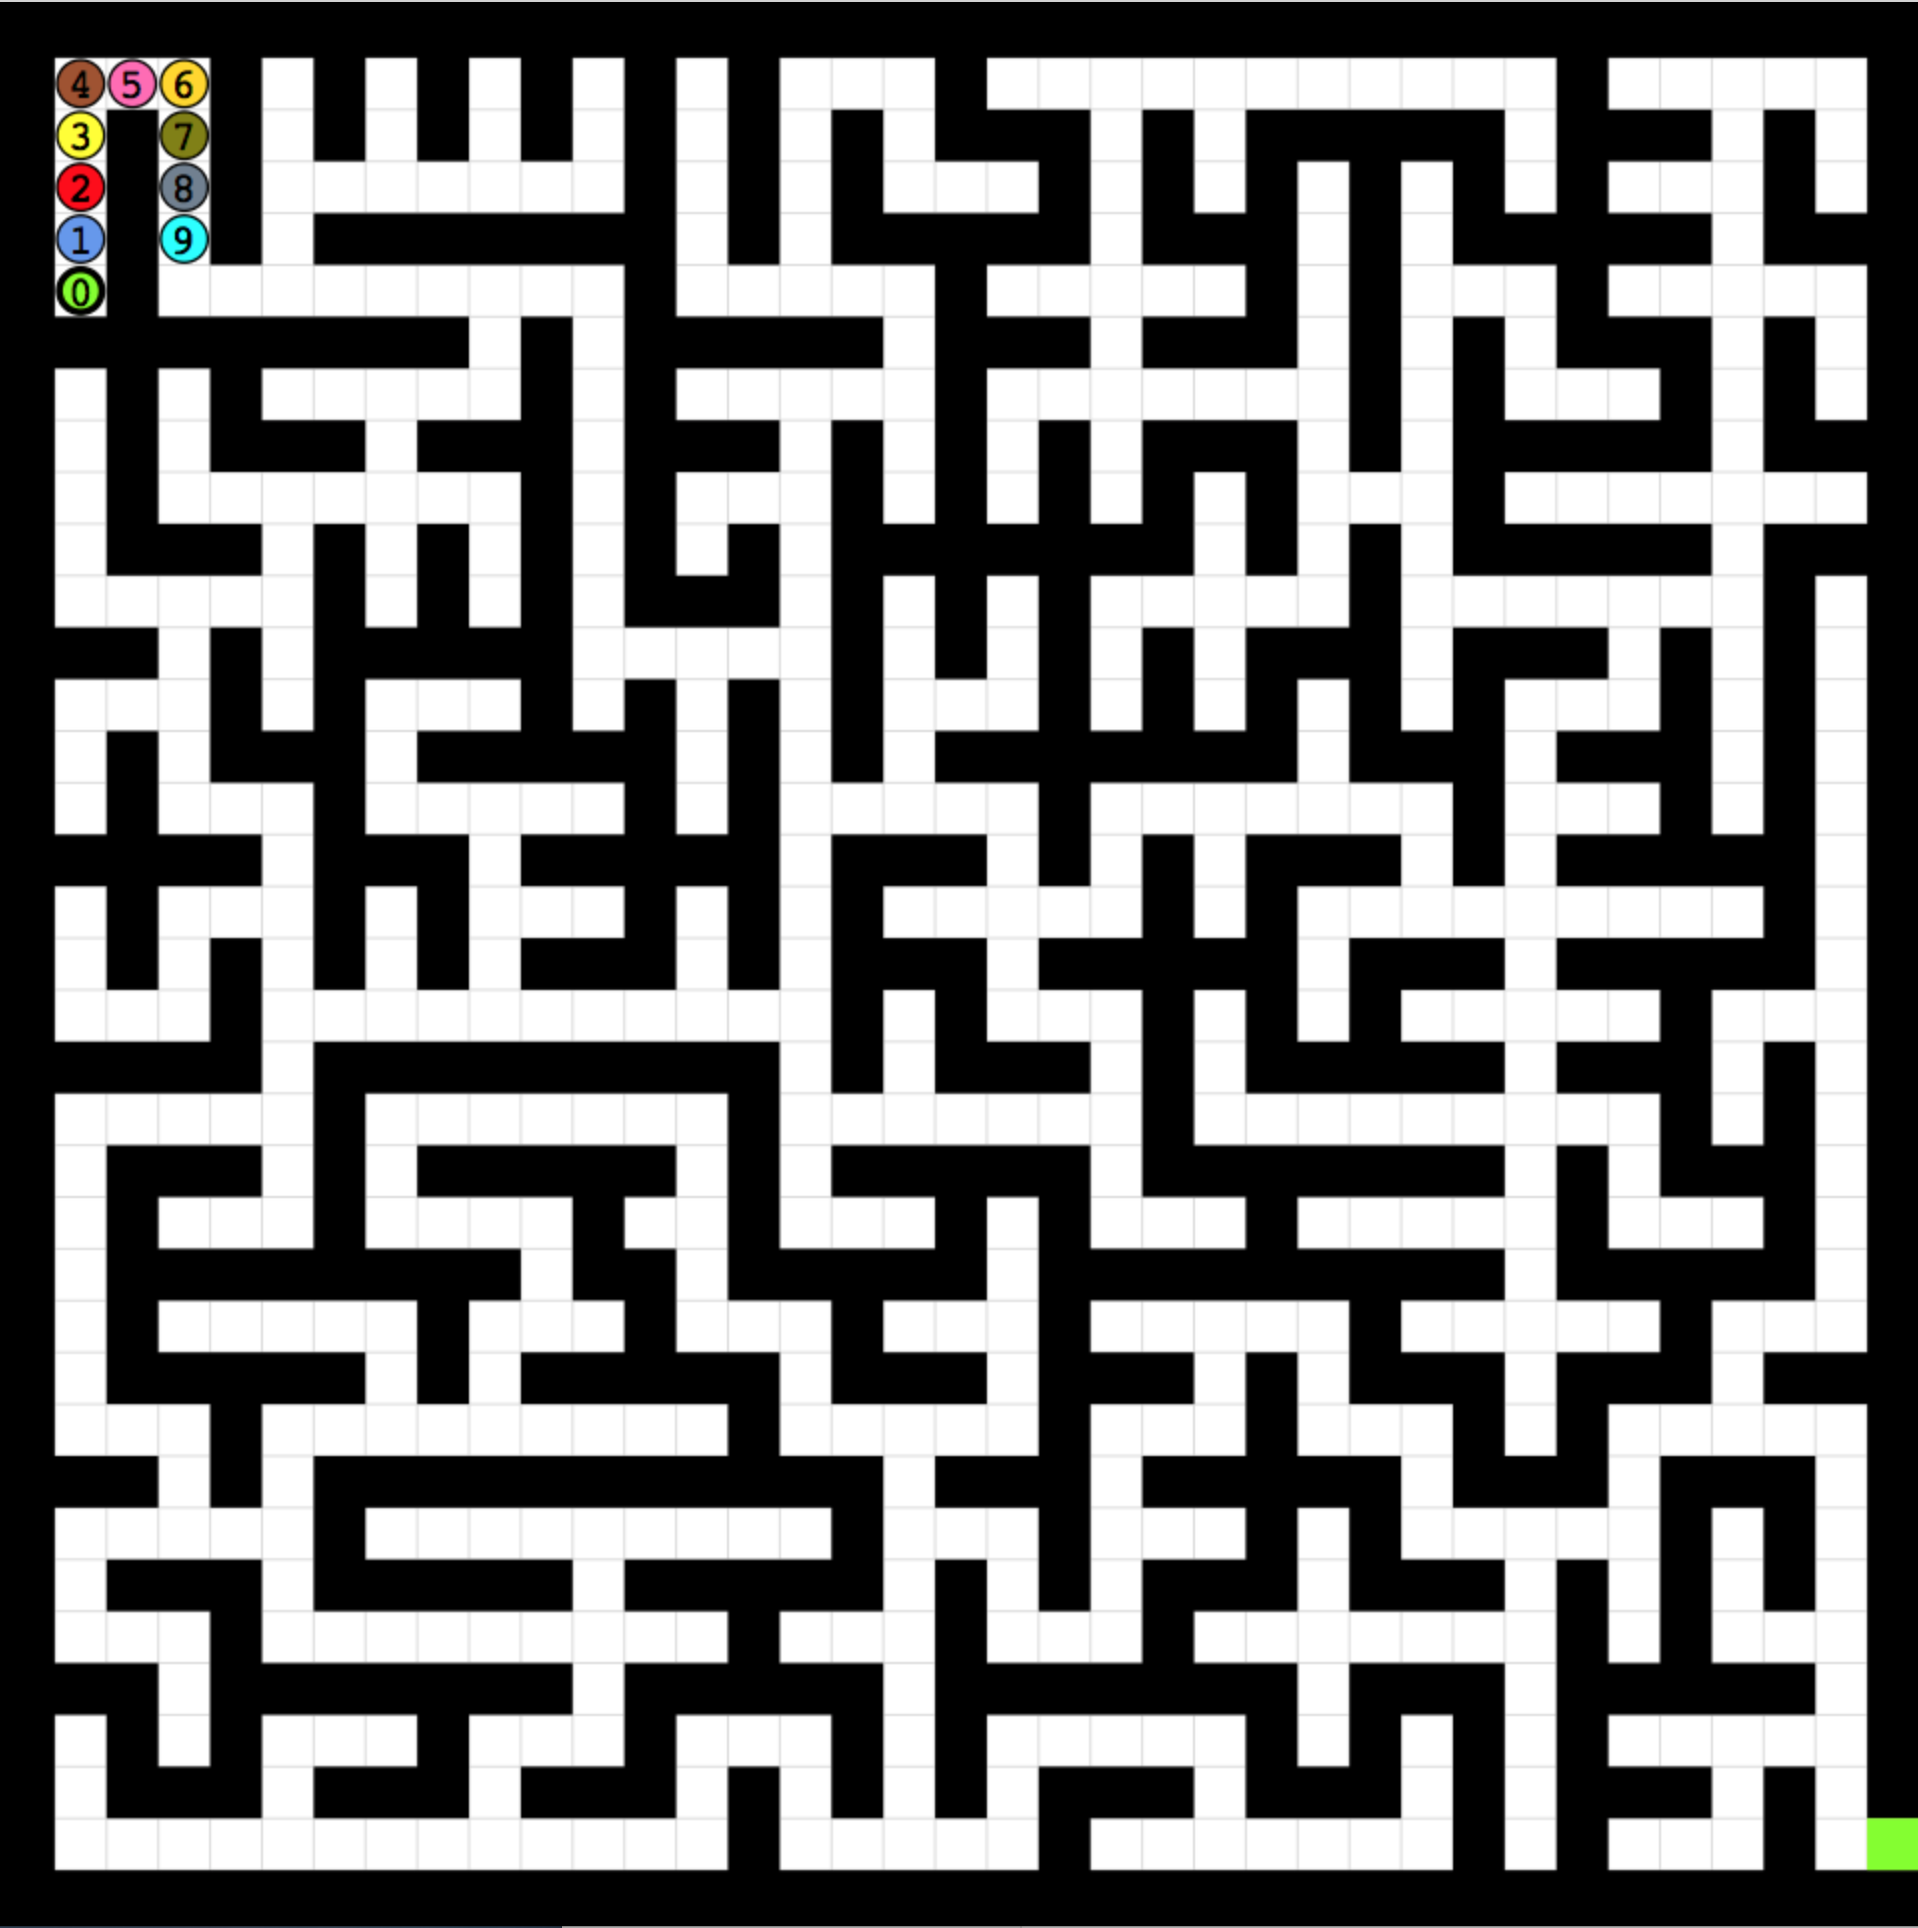
\includegraphics[height=15cm]{img/10-breakout.png}
}
\caption{En af de lidt mere udfordrende baner... (Klik på den!)}
\end{figure}

\end{document}